\begin{frame}
\frametitle{The CMS detector}\pause
\begin{center}
Silicon tracker (pixels)\\
detects charged particles going through

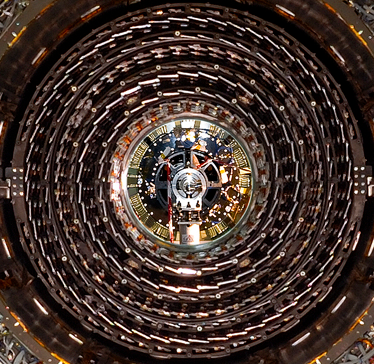
\includegraphics[width=\textwidth,height=\graphh,keepaspectratio]{/home/torterotot/Documents/PhD-Thesis/tex/slides/LHC-CMS/CMS/CMS_zoomout_pictures/CMS_slice_photo_1-trk1.png}

$\longleftarrow \SI{1}{\meter} \longrightarrow$
\end{center}
\end{frame}
\begin{frame}\addtocounter{framenumber}{-1}
\frametitle{The CMS detector}
\begin{center}
Silicon tracker (strips)\\
detects charged particles going through

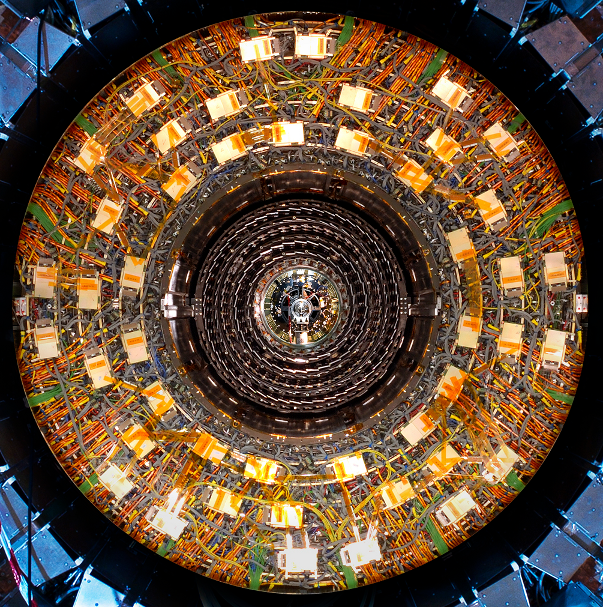
\includegraphics[width=\textwidth,height=\graphh,keepaspectratio]{/home/torterotot/Documents/PhD-Thesis/tex/slides/LHC-CMS/CMS/CMS_zoomout_pictures/CMS_slice_photo_2-trk2.png}

$\longleftarrow \SI{2}{\meter} \longrightarrow$
\end{center}
\end{frame}
\begin{frame}\addtocounter{framenumber}{-1}
\frametitle{The CMS detector}
\begin{center}
Electromagnetic calorimeter (ECAL)\\
stops photons and electrons, measure their energies

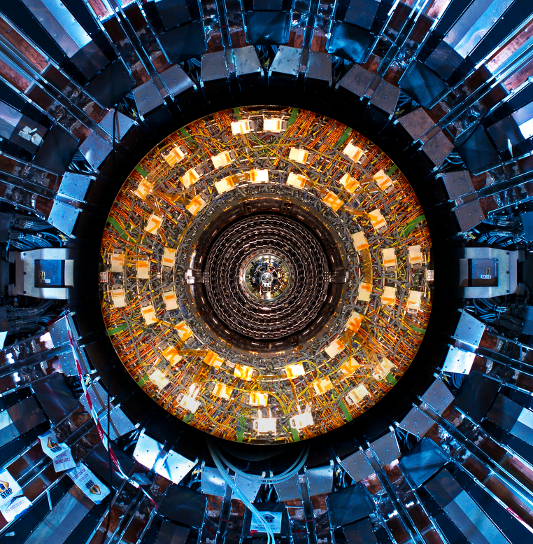
\includegraphics[width=\textwidth,height=\graphh,keepaspectratio]{/home/torterotot/Documents/PhD-Thesis/tex/slides/LHC-CMS/CMS/CMS_zoomout_pictures/CMS_slice_photo_3-ECAL.png}

$\longleftarrow \SI{3}{\meter} \longrightarrow$
\end{center}
\end{frame}
\begin{frame}\addtocounter{framenumber}{-1}
\frametitle{The CMS detector}
\begin{center}
Hadron calorimeter (HCAL)\\
stops hadrons (protons, neutrons, ...), measure their energies

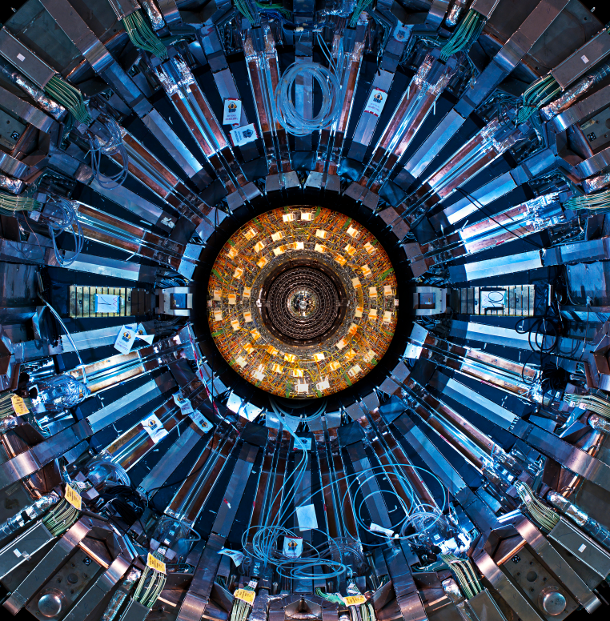
\includegraphics[width=\textwidth,height=\graphh,keepaspectratio]{/home/torterotot/Documents/PhD-Thesis/tex/slides/LHC-CMS/CMS/CMS_zoomout_pictures/CMS_slice_photo_4-HCAL.png}

$\longleftarrow \SI{5}{\meter} \longrightarrow$
\end{center}
\end{frame}
\begin{frame}\addtocounter{framenumber}{-1}
\frametitle{The CMS detector}
\begin{center}
Superconducting solenoid\\
creates a \SI{4}{\tesla} magnetic field which bends charged particles trajectories.

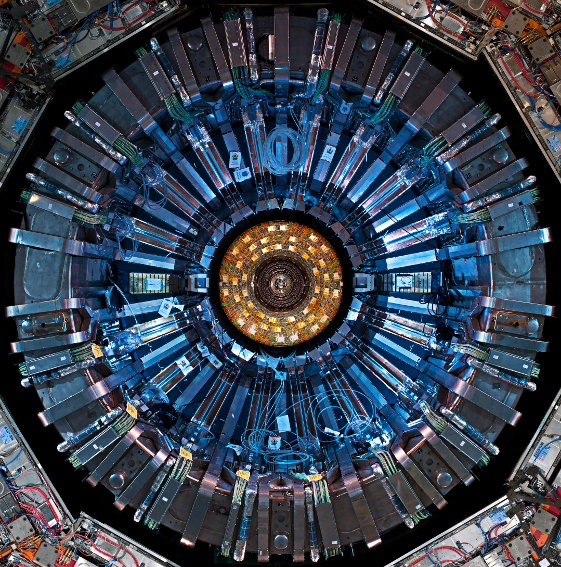
\includegraphics[width=\textwidth,height=\graphh,keepaspectratio]{/home/torterotot/Documents/PhD-Thesis/tex/slides/LHC-CMS/CMS/CMS_zoomout_pictures/CMS_slice_photo_5-solenoid.png}

$\longleftarrow \SI{7}{\meter} \longrightarrow$
\end{center}
\end{frame}
\begin{frame}\addtocounter{framenumber}{-1}
\frametitle{The CMS detector}
\begin{center}
Iron return yoke (red) interspersed with muon chambers (gray)\\
detects charged particles going through (only muons as other particles are stopped by ECAL or HCAL)

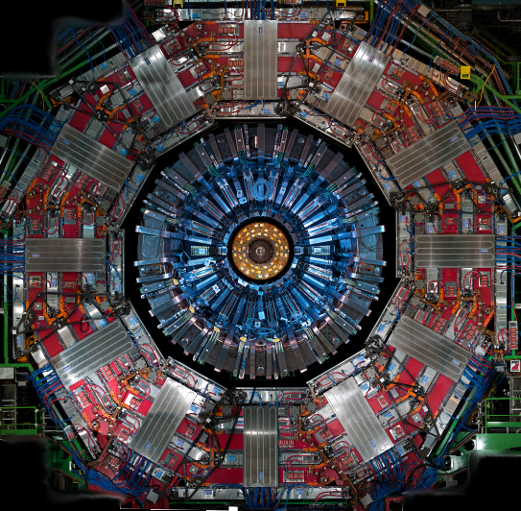
\includegraphics[width=\textwidth,height=\graphh,keepaspectratio]{/home/torterotot/Documents/PhD-Thesis/tex/slides/LHC-CMS/CMS/CMS_zoomout_pictures/CMS_slice_photo_6-muons.png}

$\longleftarrow \SI{15}{\meter} \longrightarrow$
\end{center}
\end{frame}